\chapter{Model Training Loss}
\label{appendix:training-loss}

\begin{figure}[ht]
    \centering
    \begin{subfigure}[b]{0.45\textwidth}
        \centering
        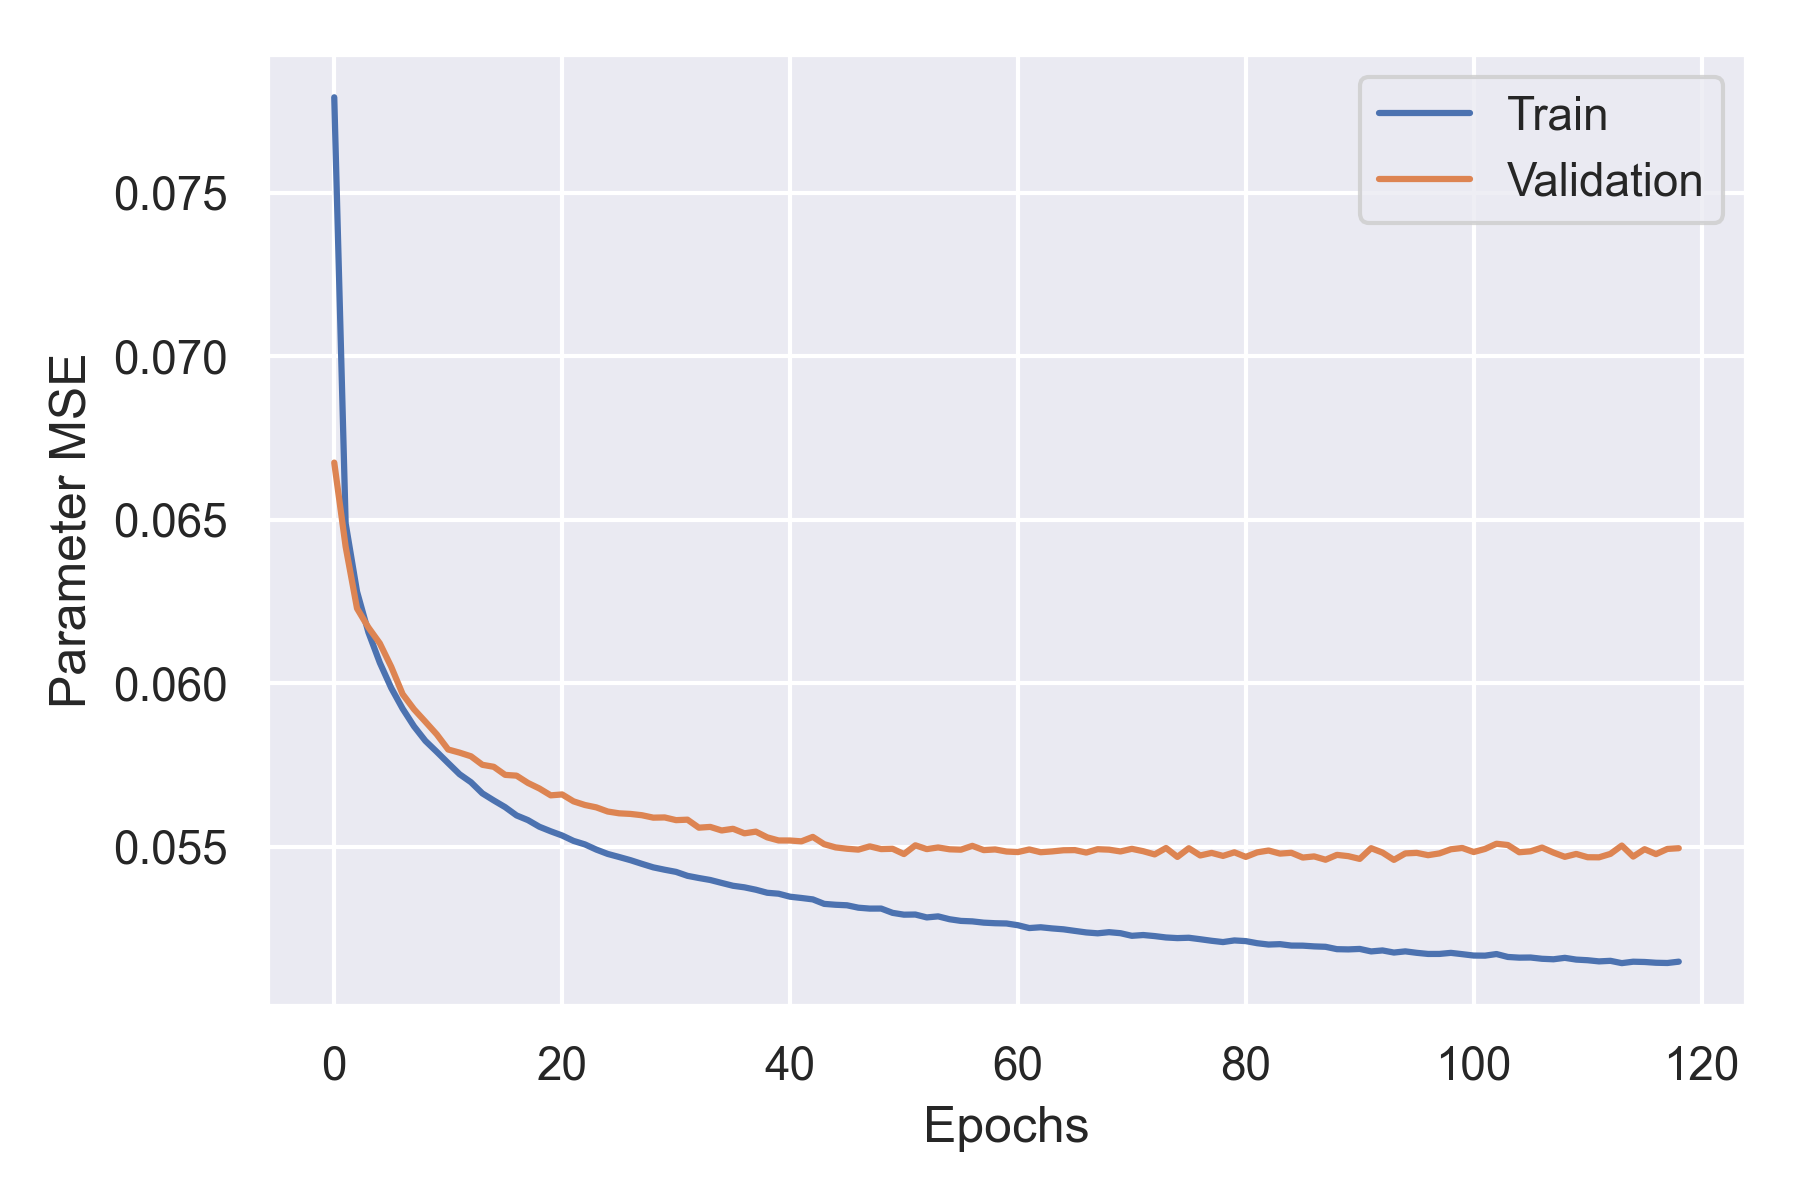
\includegraphics[width=\textwidth]{figures/inverse-synth/loss-plots/mlp-mfcc.png}
        \caption{MLP}
    \end{subfigure}
    \begin{subfigure}[b]{0.45\textwidth}
        \centering
        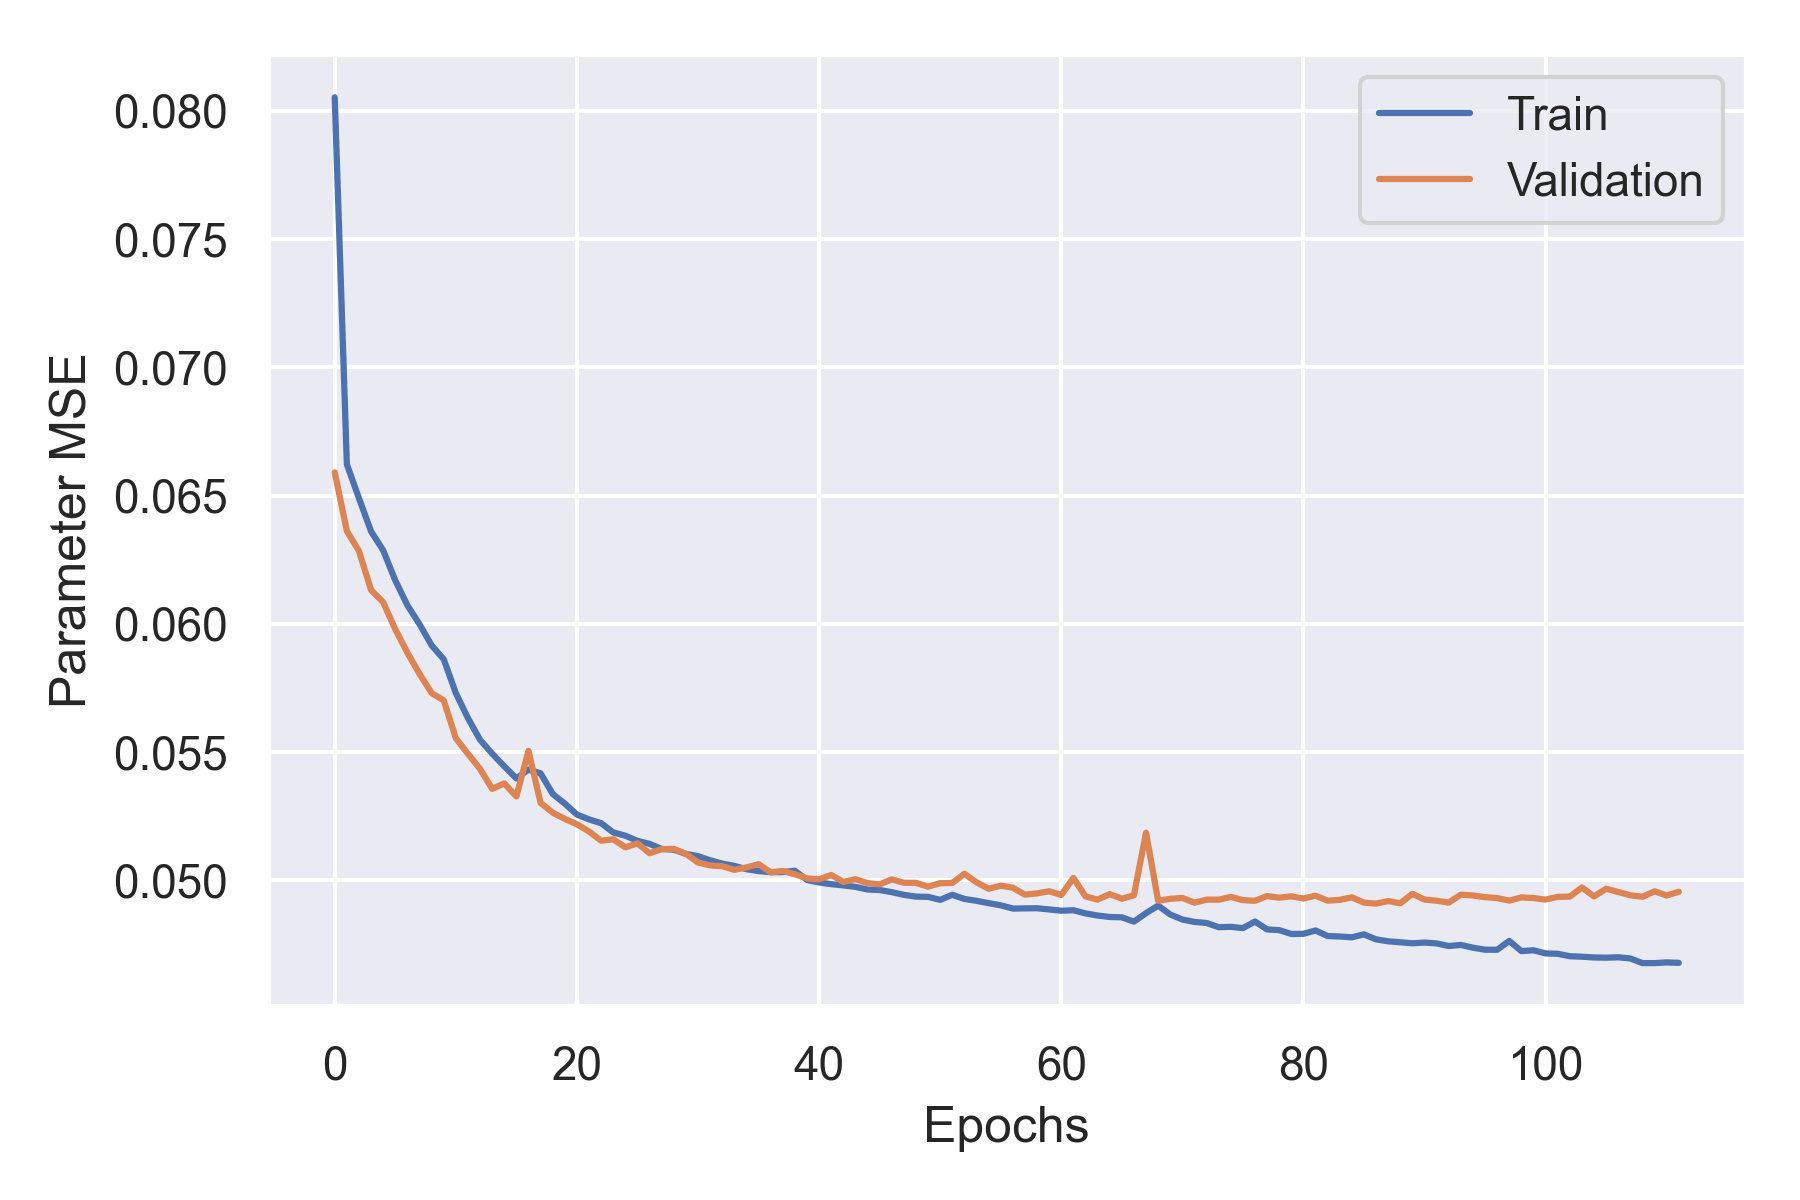
\includegraphics[width=\textwidth]{figures/inverse-synth/loss-plots/lstm-optuna-mfcc.png}
        \caption{LSTM}
    \end{subfigure}
    
    \vspace{1cm}
    
    \begin{subfigure}[b]{0.45\textwidth}
        \centering
        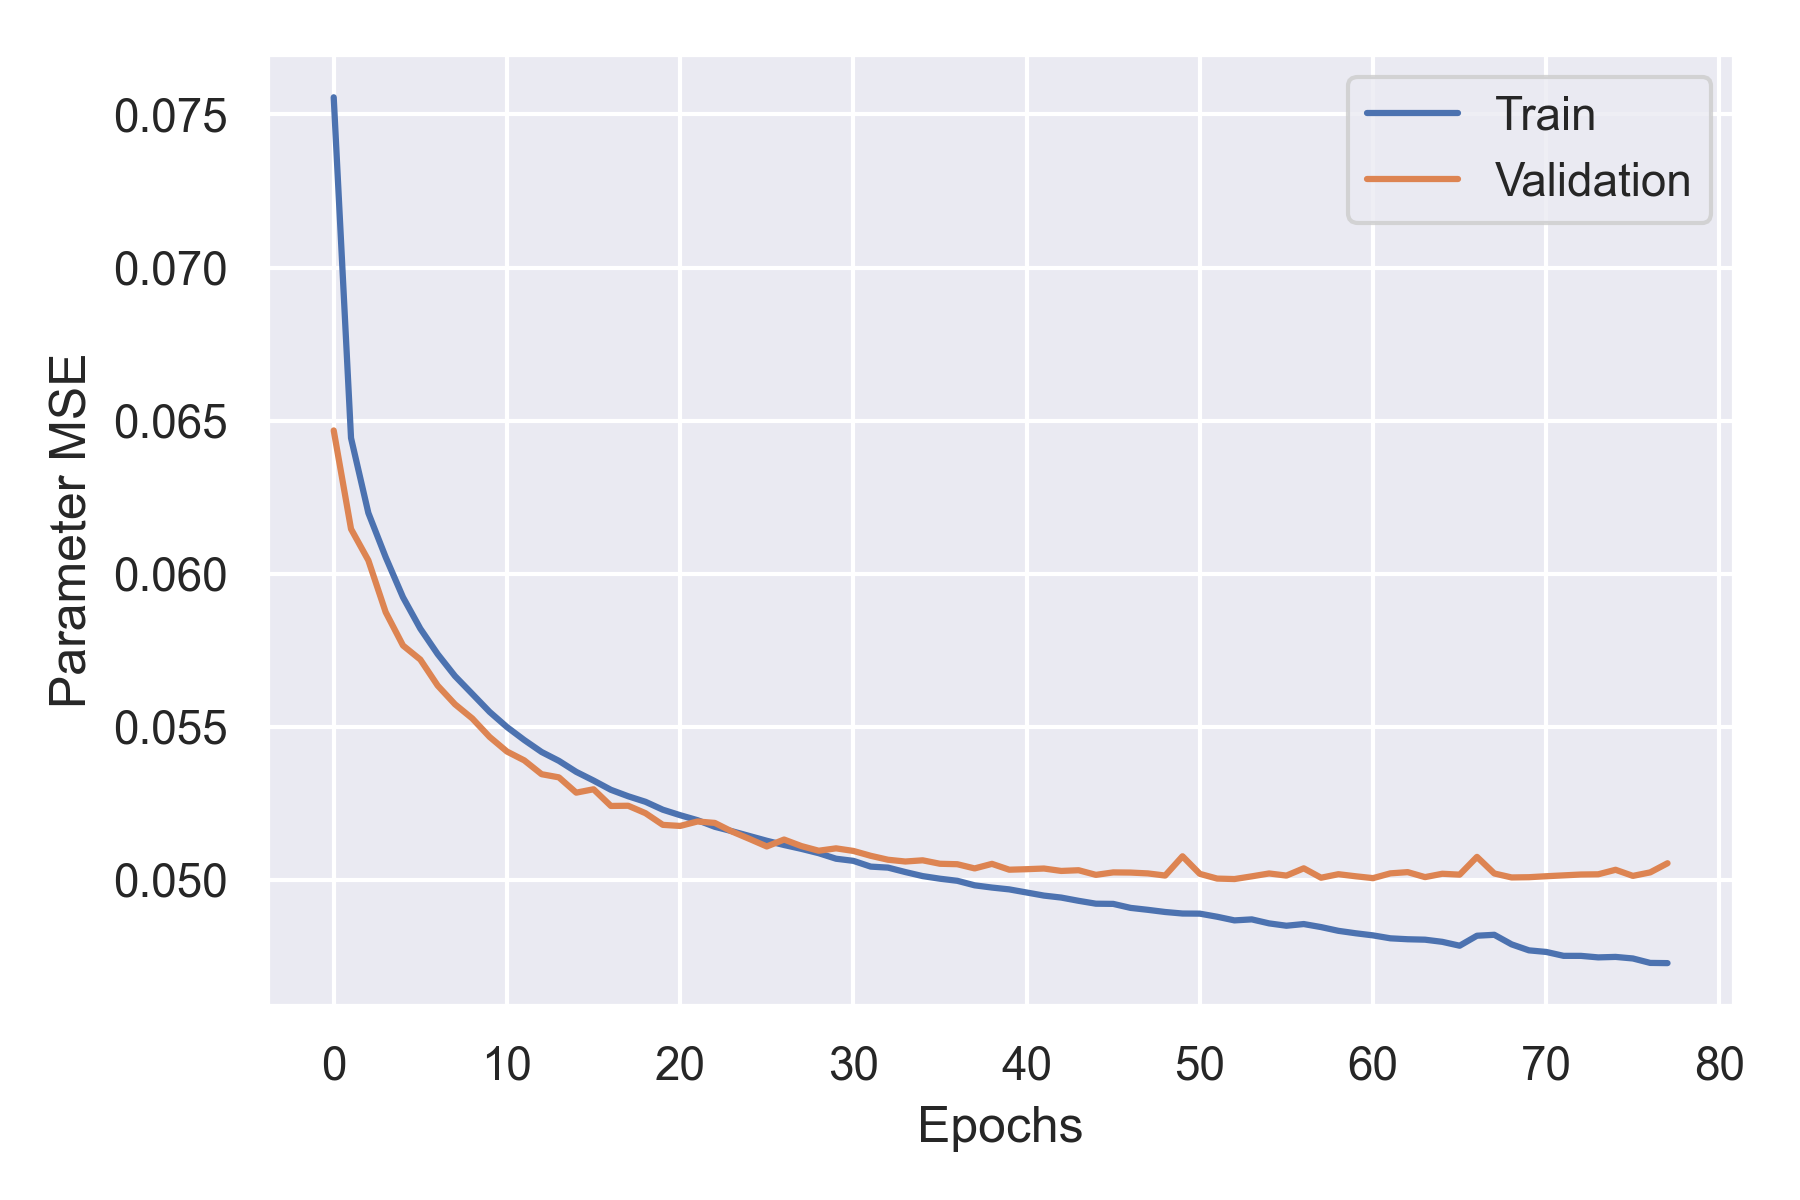
\includegraphics[width=\textwidth]{figures/inverse-synth/loss-plots/bilstm-mfcc.png}
        \caption{LSTM++}
    \end{subfigure}
    \begin{subfigure}[b]{0.45\textwidth}
        \centering
        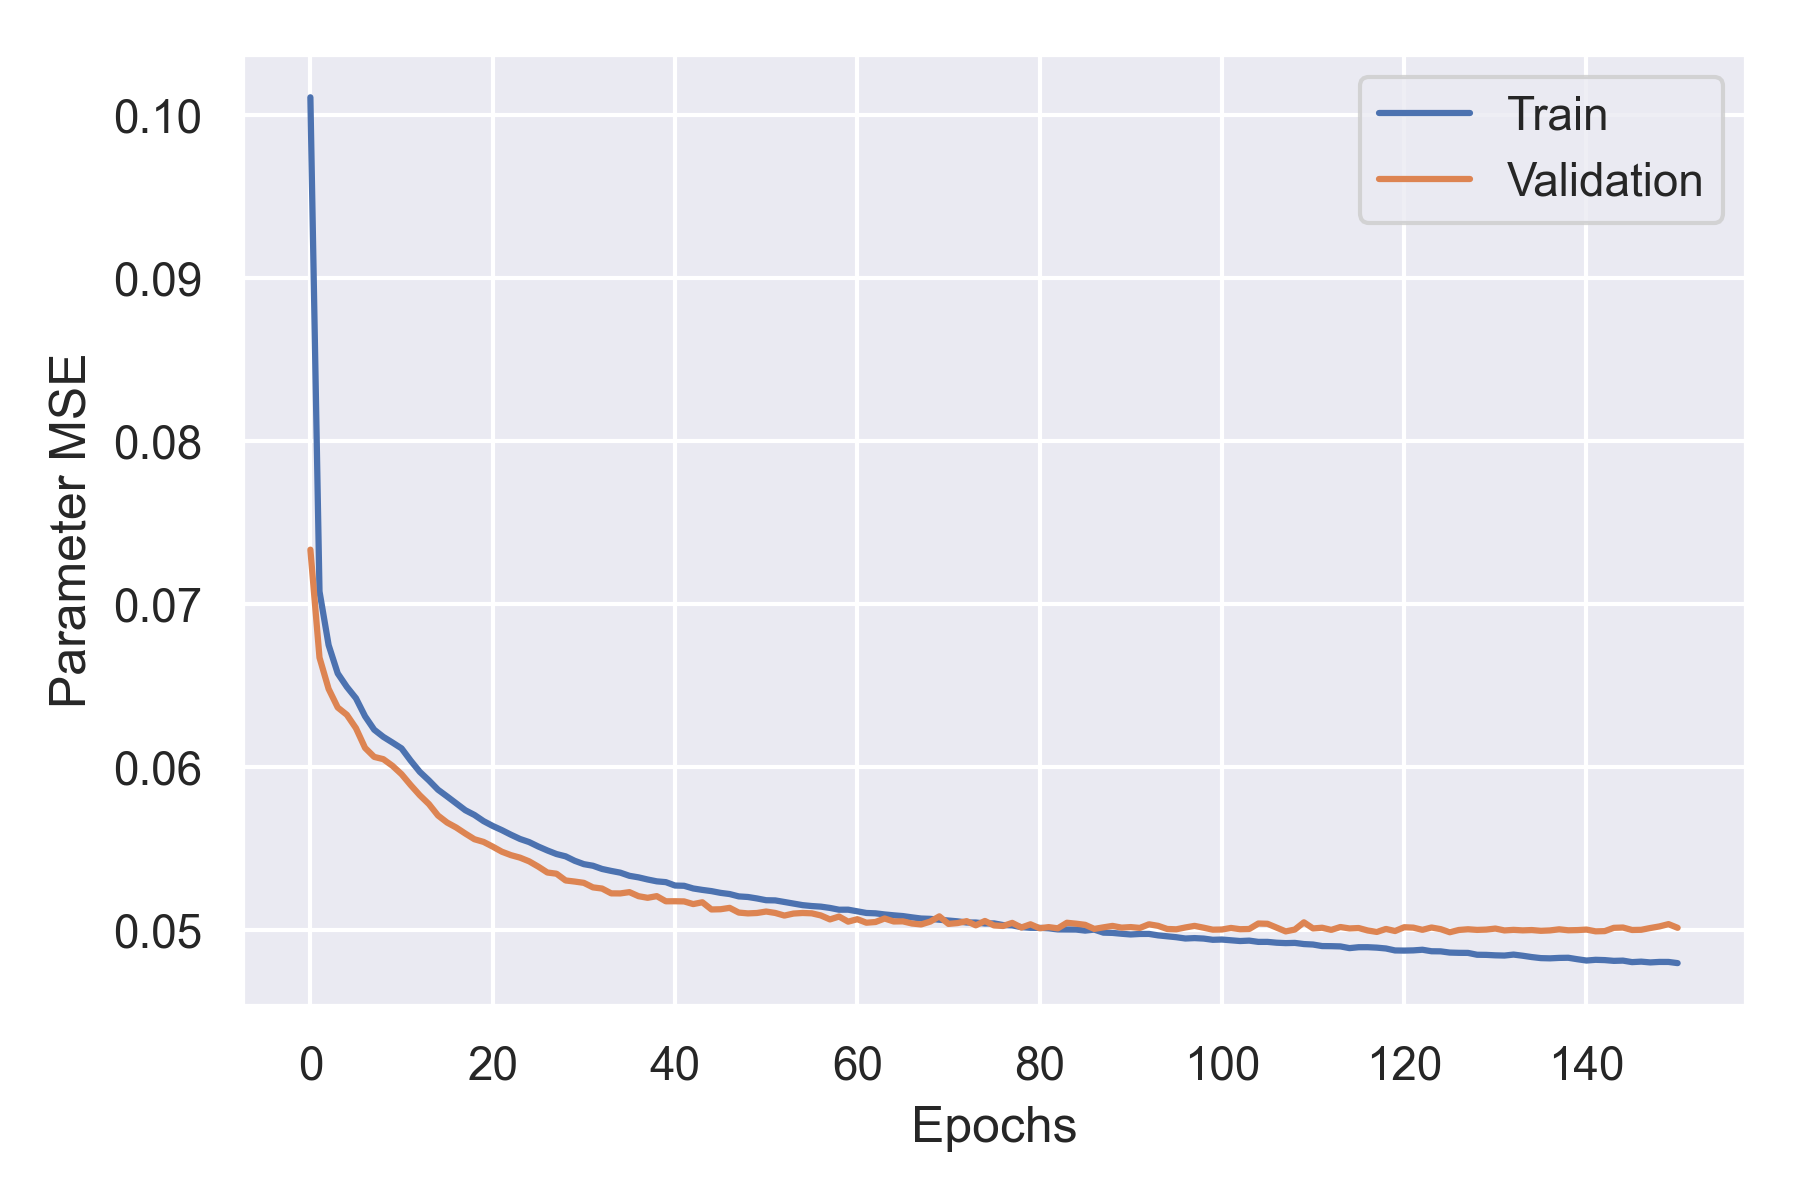
\includegraphics[width=\textwidth]{figures/inverse-synth/loss-plots/bilstm-optuna-mfcc.png}
        \caption{5-LSTM++}
    \end{subfigure}
\end{figure}

\begin{figure}[t]\ContinuedFloat
    \begin{subfigure}[b]{0.45\textwidth}
        \centering
        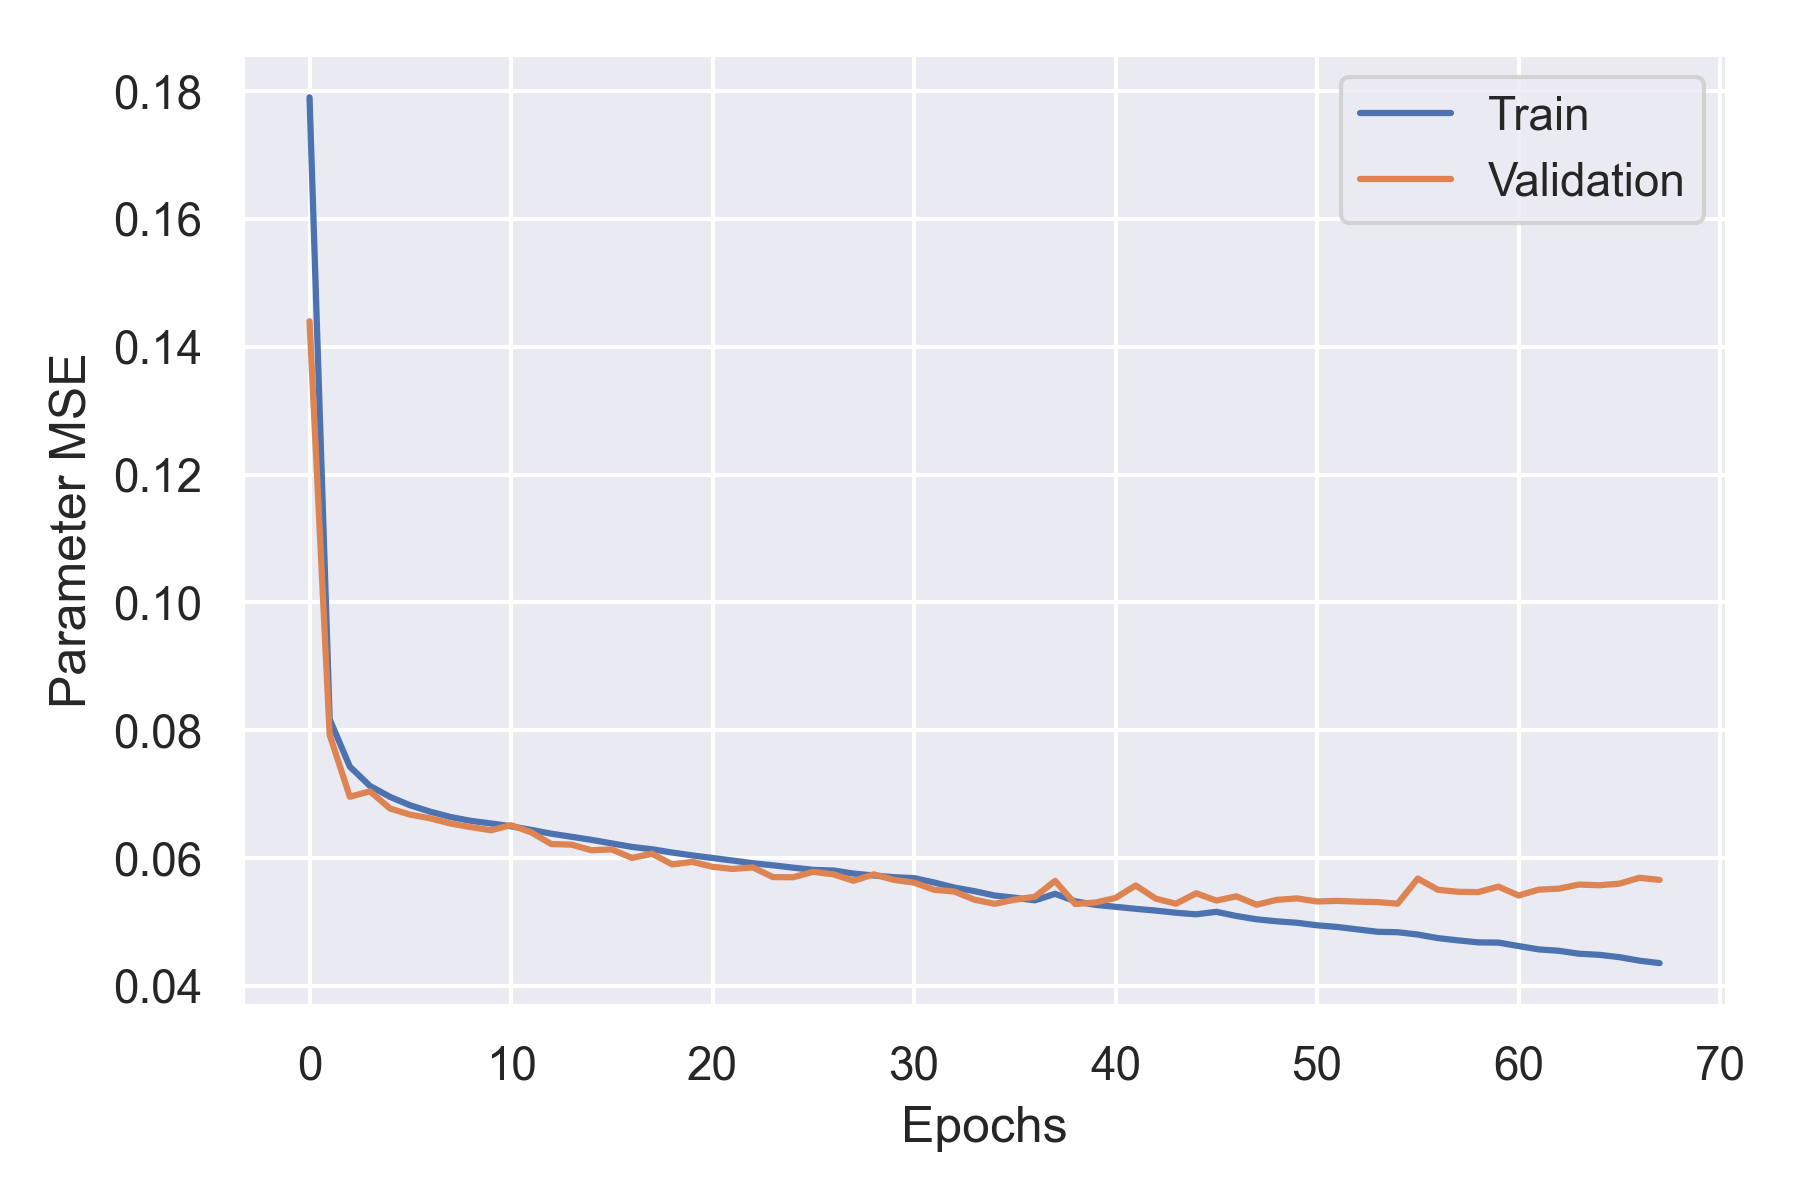
\includegraphics[width=\textwidth]{figures/inverse-synth/loss-plots/conv6-mel.png}
        \caption{Conv6}
    \end{subfigure}
    \begin{subfigure}[b]{0.45\textwidth}
        \centering
        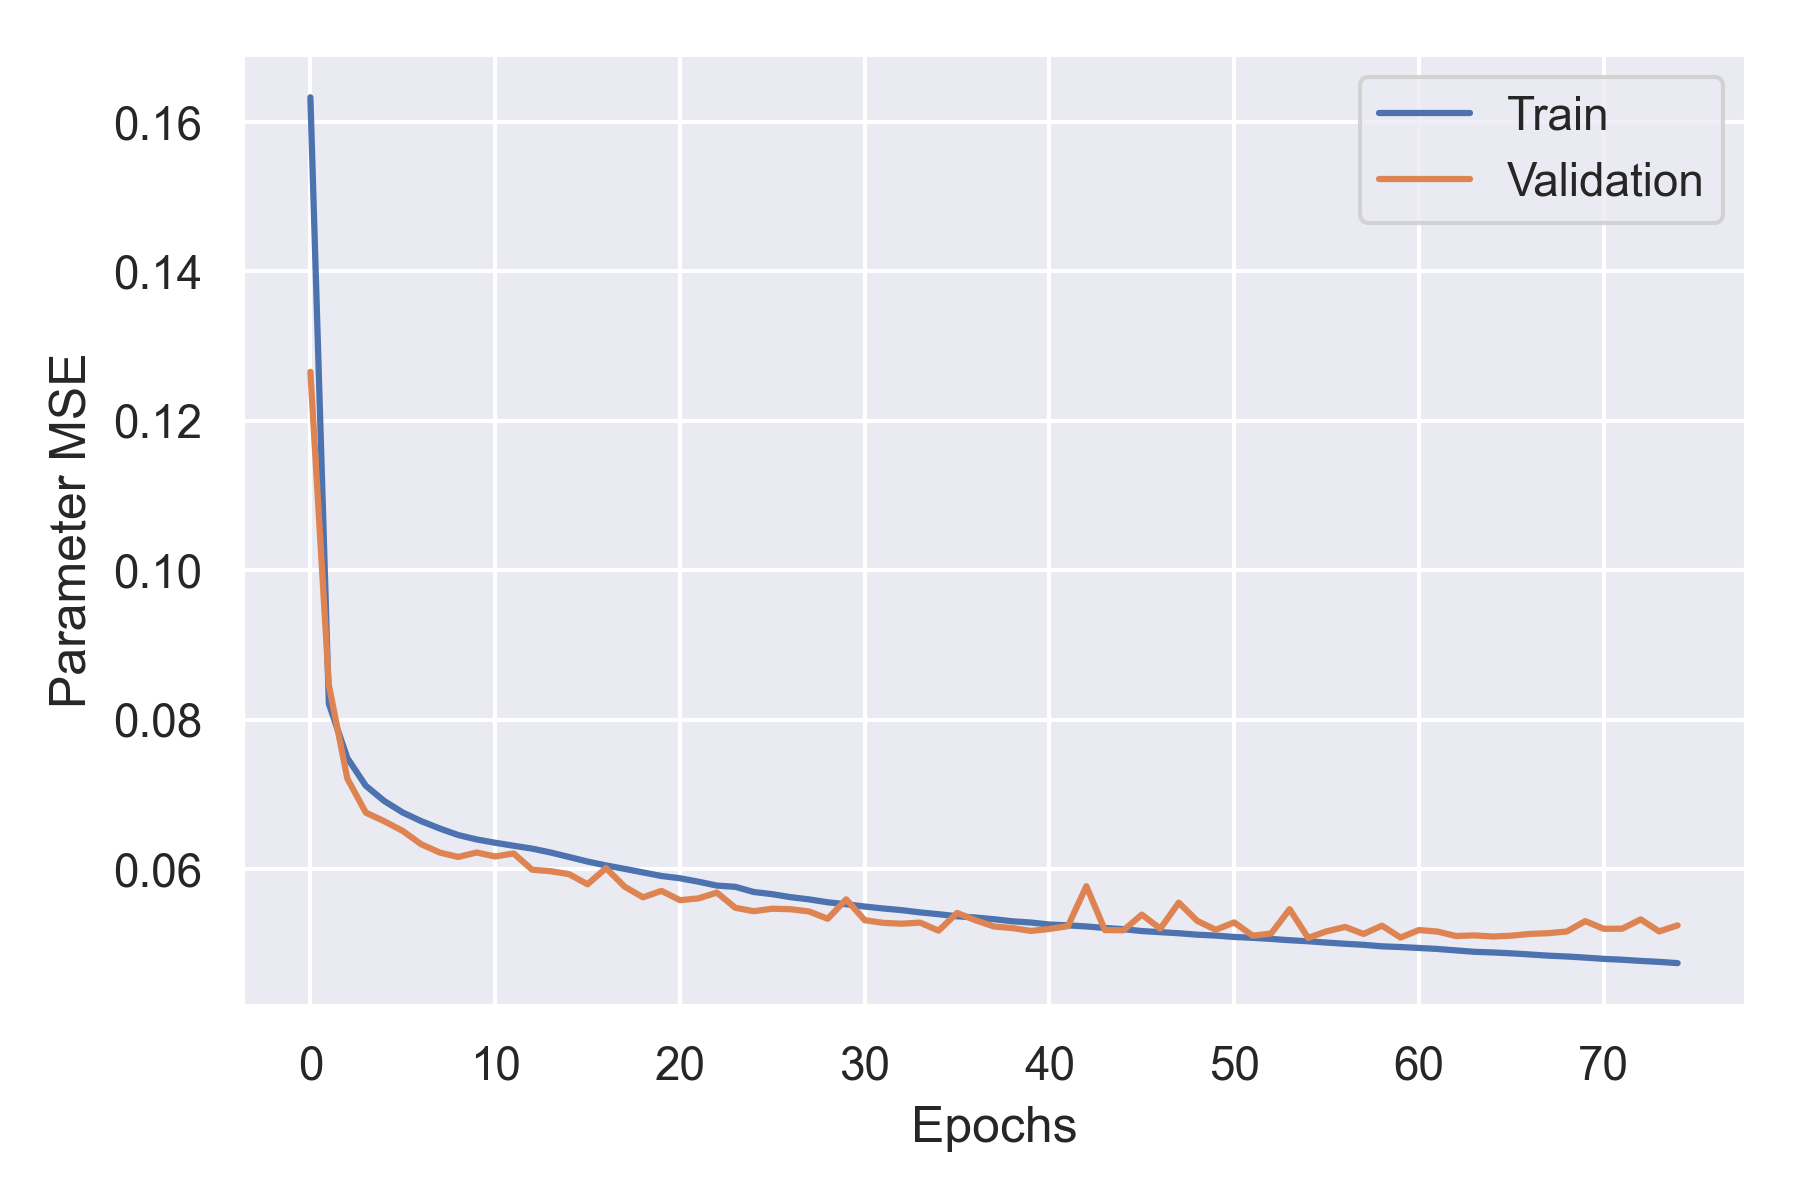
\includegraphics[width=\textwidth]{figures/inverse-synth/loss-plots/conv6s-mel.png}
        \caption{Conv6s}
    \end{subfigure}
    
    \vspace{1cm}
    
    \begin{subfigure}[b]{0.45\textwidth}
        \centering
        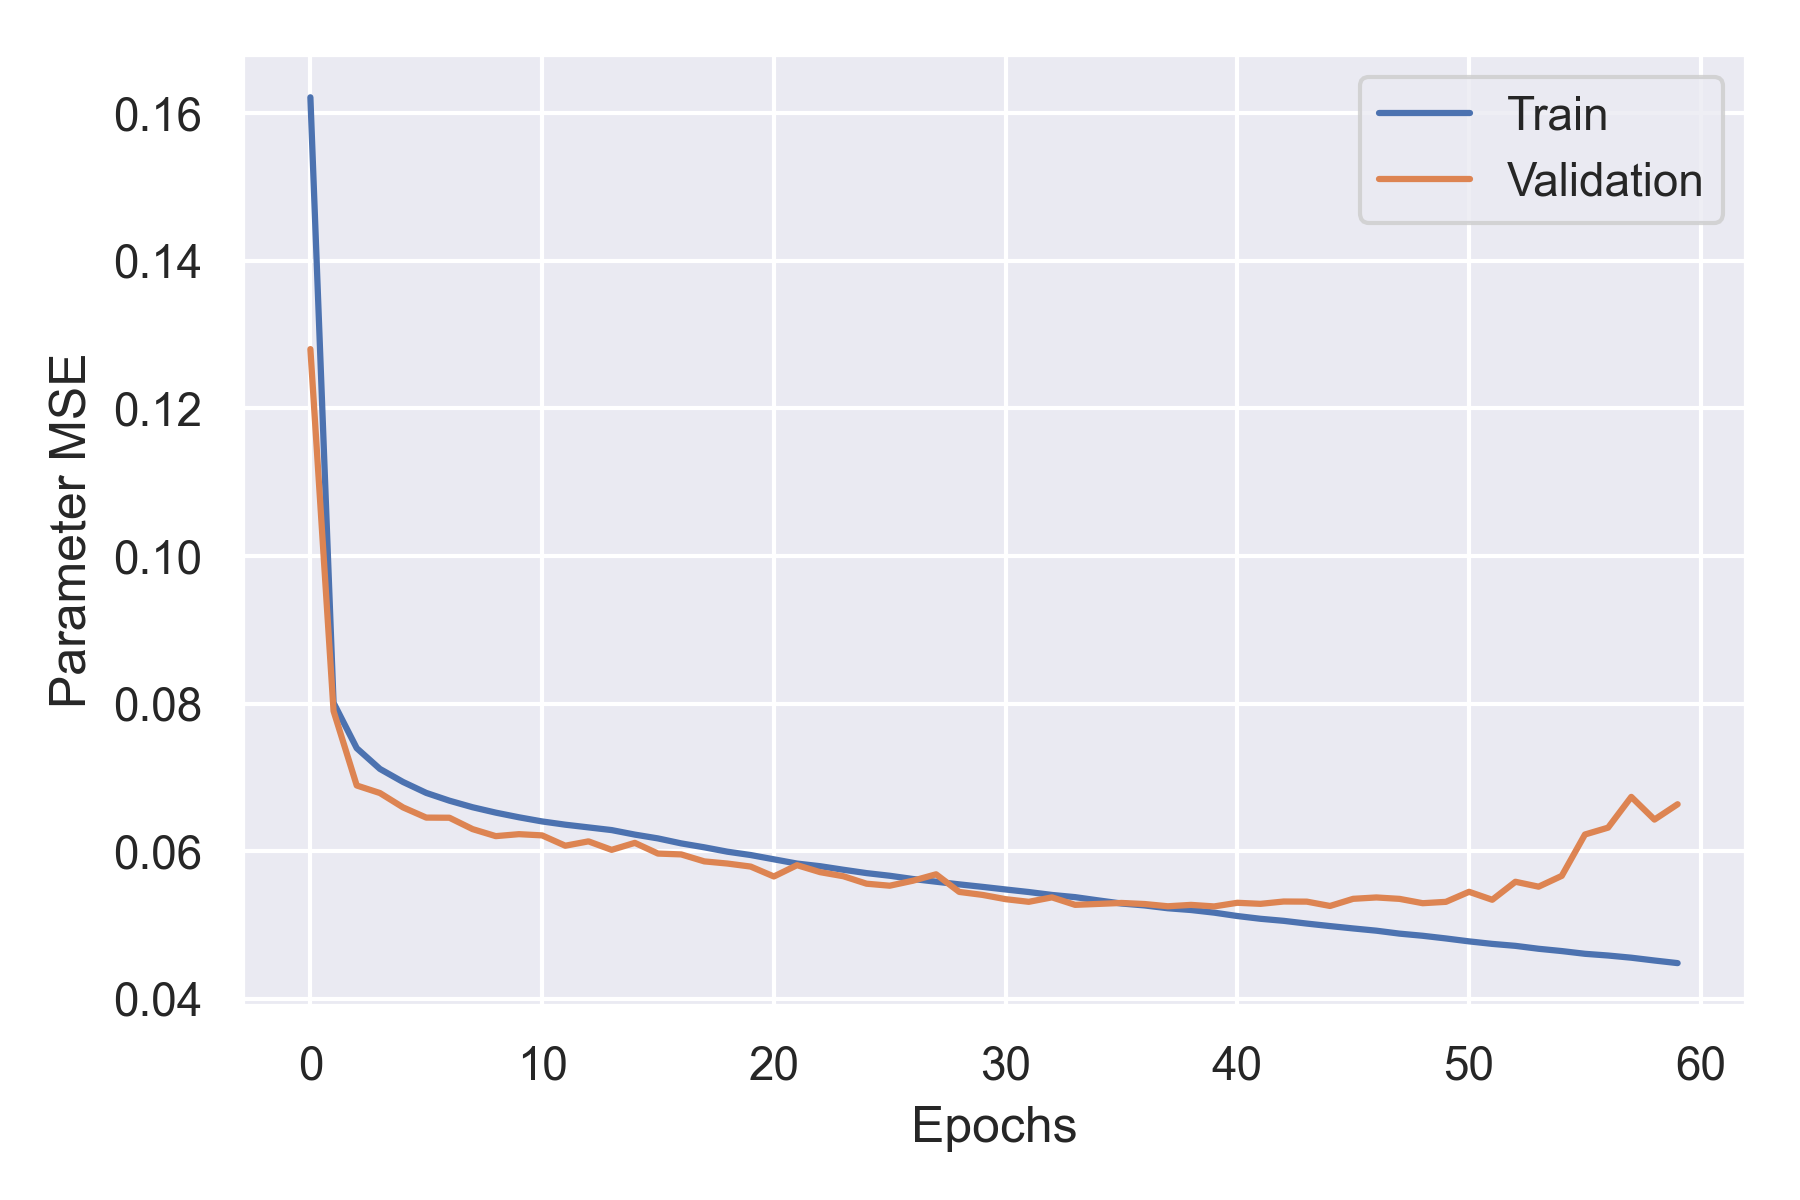
\includegraphics[width=\textwidth]{figures/inverse-synth/loss-plots/conv5-mel.png}
        \caption{Conv5}
    \end{subfigure}
    \begin{subfigure}[b]{0.45\textwidth}
        \centering
        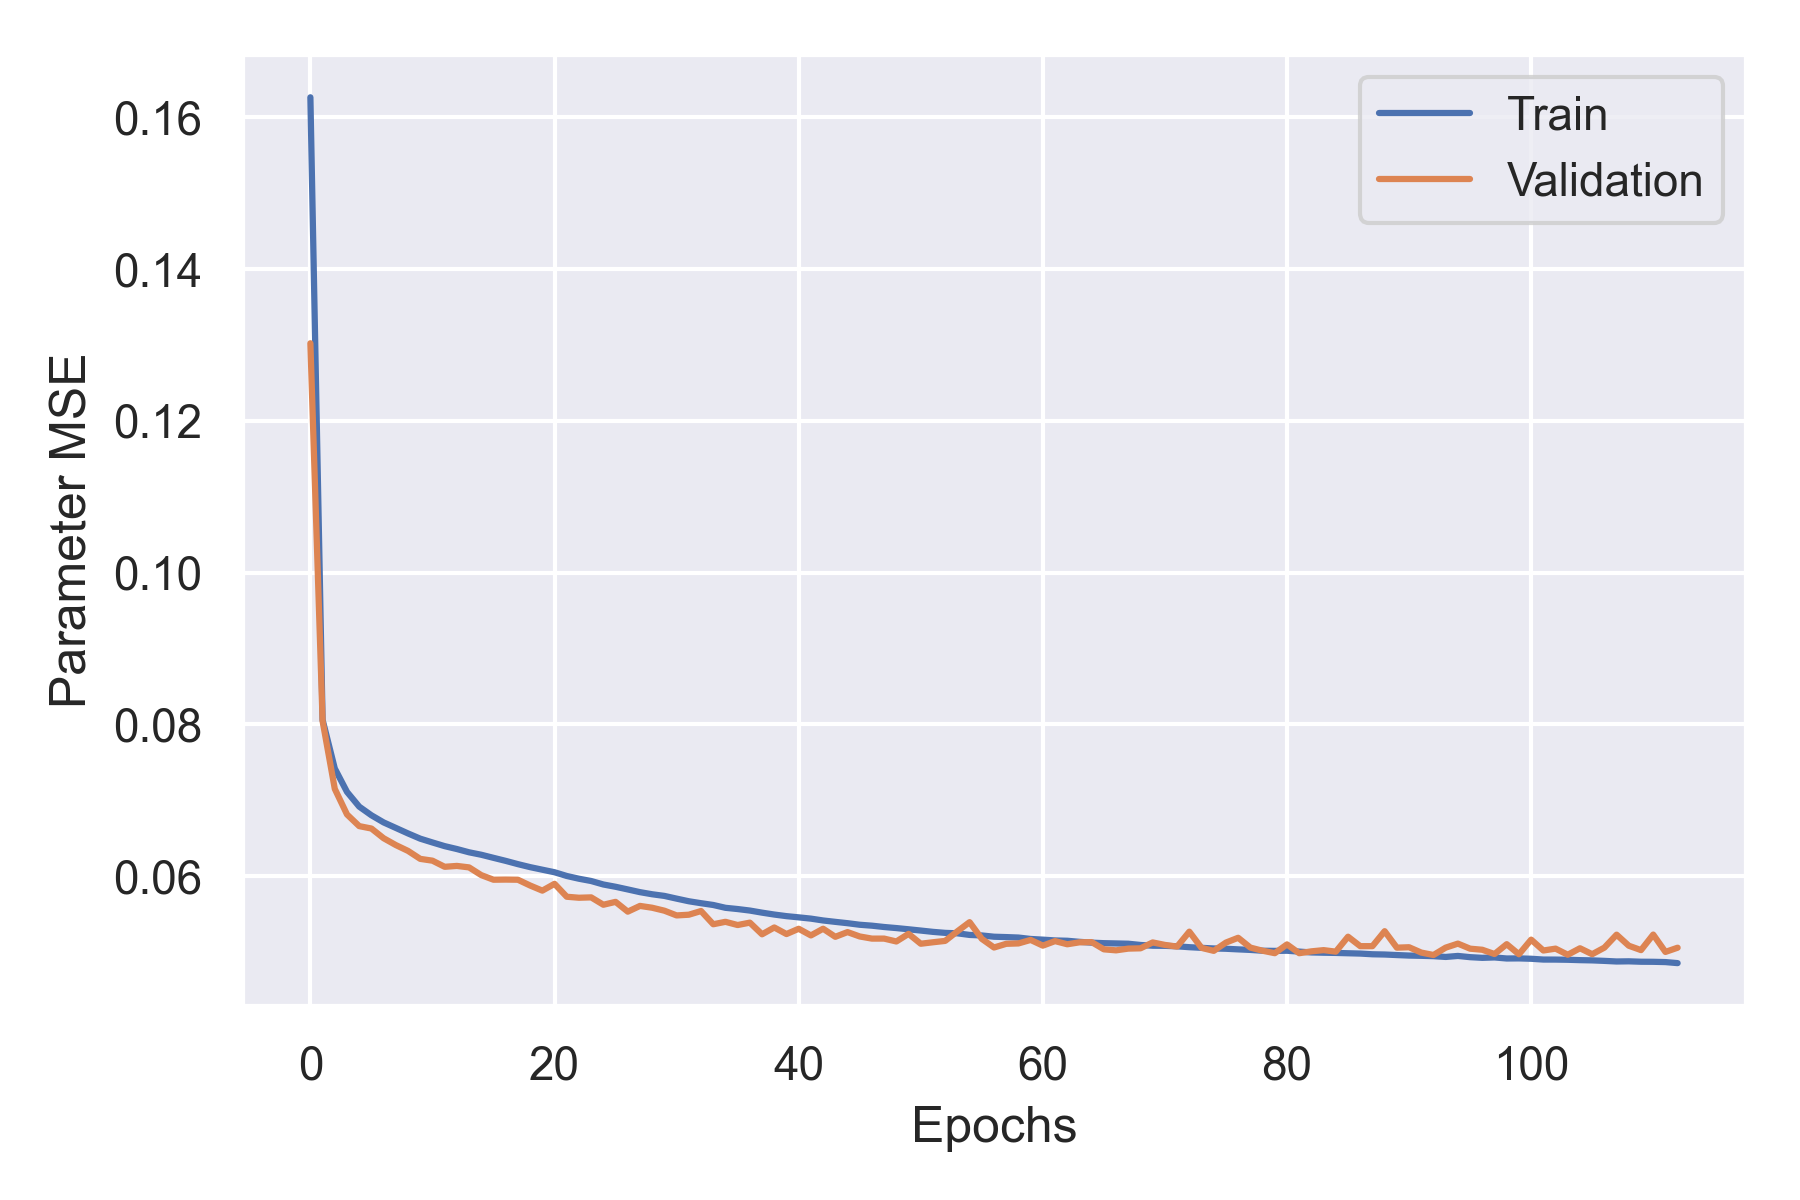
\includegraphics[width=\textwidth]{figures/inverse-synth/loss-plots/conv5s-mel.png}
        \caption{Conv5s}
    \end{subfigure}
\end{figure}